\documentclass[10pt]{article}
\usepackage{tikz}
\usetikzlibrary{fit}
\begin{document}

%use for sets with non-alphanumeric characters
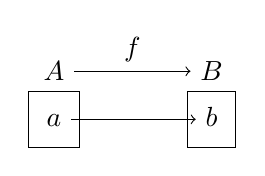
\begin{tikzpicture}
  \foreach[count=\i] \set/\elements in {$A$/{$a$}, $B$/{$b$}} { %domain and co-domain
  \begin{scope}[local bounding box=\set, x=2cm, y=0.5cm]
    \foreach[count=\j] \element in \elements {
      \node[minimum width=1em,anchor=base,text height=1.4ex,text depth=0.25ex]
      (\i-\j) at (\i,-\j) {\element};
    }
  \end{scope}
  \node[draw, fit=(\set), label={[name=\i]above:\set}] {};
  }
  \foreach \domain/\target in {1/1} { %function pairs, uses indices
      \draw[->] (1-\domain) -- (2-\target);
    }
  \draw[->] (1) -- node[above]{$f$}(2); %function name
\end{tikzpicture}

%use for sets for only alphanumeric characters
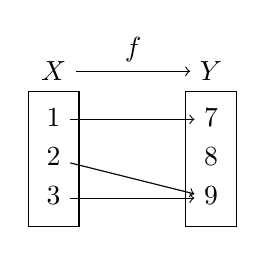
\begin{tikzpicture}
  \foreach[count=\i] \set/\elements in {X/{1,2,3}, Y/{7,8,9}} { %domain and co-domain
  \begin{scope}[local bounding box=\set, x=2cm, y=0.5cm]
    \foreach[count=\j] \element in \elements {
      \node[minimum width=1em,anchor=base,text height=1.4ex,text depth=0.25ex]
      (\i-\element) at (\i,-\j) {$\element$};
    }
  \end{scope}
  \node[draw, fit=(\set), label={[name=\i]above:$\set$}] {};
  }
  \foreach \domain/\target in {1/7,2/9,3/9} { %function pairs, uses indices
      \draw[->] (1-\domain) -- (2-\target);
    }
  \draw[->] (1) -- node[above]{$f$}(2); %function name
\end{tikzpicture}

%use for digraphs for center
\begin{tikzpicture}
  \foreach[count=\i] \element in {a,b,c,d} { %domain
      \node (\element) at (\i * 360 / 4 + 90:2) {$\element$};
      \node (\element') at (\i * 360 / 4 + 90:3) {};
    }
  \foreach \j/\l in {a/b, b/c, c/d, e/b, e/a} { %a to b
      \draw[->] (\j) -- (\l);
    }
  \foreach \j/\l in {a/a} { %a to a
      \draw[--] (\j) to[bend right=90] (\j');
      \draw[->] (\j') to[bend right=90] (\j);
  }
\end{tikzpicture}
\end{document}